
\chapter{Ambiente de execu��o}
\label{cap:ambiente}


% Describe the execution engine based on EMF. This section corresponds to the implementation section that goes in most papers. Make it clear in the text that it is the implementation.

%% Describe why the execution environment is needed
%- The  metamodel allows for us to define a Broker layer...
%- but in order to execute it so that it is capable of handling requests from the middleware layer ...
%- we developed an execution engine (that therefore provides dynamic semantics to the  metamodel)
Though the  metamodel provides abstractions that enable the description of a broker layer, it is not enough to have an executable layer, capable of handling requests at runtime. In order to fill in this gap, we developed an execution environment that loads a broker layer model and behaves accordingly, therefore providing operational semantics for the proposed  metamodel.


%% MAKE IT CLEAR that the execution engine loads the XMI models defined by using EMF
%- The execution environment loads a Broker layer model defined as an EMF XMI file.
%- Based on this model, the execution environment initializes a Broker layer for a DSML execution engine.
%- It uses the classes generated by EMF from the  metamodel to process the model.
The provided execution environment was developed in the Java platform and comprises components for executing a broker layer model and a library for interfacing with the resources to be managed by the layer. It loads a model described in EMF XMI 2.0 and initializes a broker layer for a DSML execution engine.

% Introduction to understand the following paragraphs
%in this section we deal with the actual implementation that actually process the requests driven by a given Broker model
%- The name of the classes are overloaded (always refer to the implementation exception when mentioned)
%- The architecture resembles the  metamodel
In this section, we describe the implementation of this execution environment, including its main components and how they interact in order to provide the behavior described by the model loaded in it. Though the names employed for describing these components may be the same used for elements of the  metamodel they are not the same. The components described here are part of the actual Java implementation but are related to their homonymous in the  metamodel.

% Describe the overall flow of the execution environment
Under the implemented execution environment, a broker layer constantly waits for calls from the upper layer or events from resources, that once arrived are enqueued for later processing. In order to process a signal, the appropriate handler is found and executed. In accordance with the model, the handler executes the associated action that may interact with resources and manipulate the state maintained by the layer. Specialized handlers are also set up for handling signals that may activate self-management functions.

The figure ~\ref{fig:environment} illustrates the
%flow of control for 
main elements that compose
a broker layer at runtime. The \emph{Broker Manager} is the main element of the execution environment which is the responsible for controlling the flow of execution. It is a runtime object that realizes a \textsf{Manager} described in the  metamodel.
%Therefore, at runtime a \emph{Broker Manager] may also be used as a resource for another \emph{Broker Manager}  and so on

\begin{figure*}
 \centering
 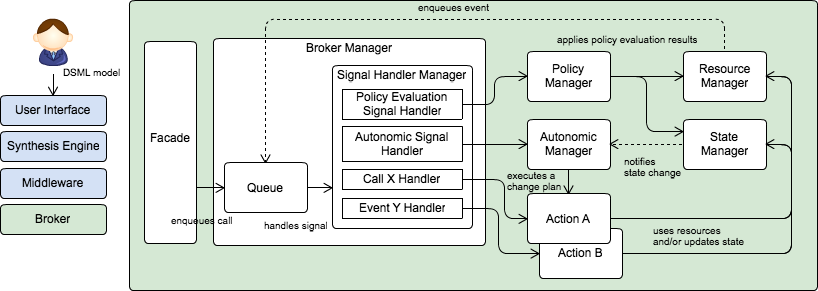
\includegraphics[width=0.7\textwidth]{environment}
 \caption{Execution environment for the broker layer}
 \label{fig:environment}
\end{figure*}

A \emph{Broker Manager} serializes the handling of signals by enqueueing them and afterwards processing them one at a time. Once a signal is dequeued, it is processed by the \emph{Signal Handler Manager} that identifies and executes the correct handler for the given signal. The \emph{Signal Handler Manager} maintains a registry of \emph{Signal Handlers} and searches for the first that is capable of handling the given signal. \emph{Signal Handlers} in the registry are loaded from the handlers and actions defined in the executing model, in conformance to the equivalent  metamodel constructs mentioned earlier.

%signals/events
%handlers registered into the SignalHandlerManager
Besides those, the specialized \emph{Autonomic Signal Handler} and \emph{Policy Evaluation Signal Handler} are also set up for monitoring signals that may be of interest for self-management. \emph{Autonomic Signal Handler} checks if a signal is related to any of the symptoms that are to be monitored and if positive sends the signal information to the \emph{Autonomic Manager} that may then execute its functions. The \emph{Policy Evaluation Signal Handler}, in turn, verifies if a signal is defined as a policy evaluation point and requests the \emph{Policy Manager} to start the policy evaluation process. Regardless of their result, these specialized handlers leave the signal flagged as not handled, so that it can be handled by an action defined in the model. An action


The \emph{Resource Manager} provides an interface for querying and obtaining its managed resources. These resources are returned as instances of \textsf{Resource}. \textsf{ManagedResource} is a subtype of \textsf{Resource} and wraps the actual resource along with its metadata. \textsf{BrokerManager} is the other subtype of \textsf{Resource}, which allows a \emph{Broker Manager} to be employed as a resource.
In order to be managed by a broker layer, resources should implement the \textsf{Manageable} interface and annotate their provided calls with a \textsf{@Call} annotation. Resources should also use the provided class \textsf{Event} to signal an event to be handled by the layer. The \emph{Resource Manager} interacts with a resources through a touchpoint which serializes calls to a resource and handles the events signaled by resources.
% Also expose the setEventListener method
% Main manager registers into the resource manager as a listener of the resource events

In a similar way, the \emph{State Manager} provides an interface for creating and querying registers for the data types described in the  metamodel. A data register is represented by the class \textsf{StateHolder} that provides methods for obtaining the values for its attributes and subtypes.
% autonomic manager registers into the state manager as a listener of state changes

%Both state and resource managers are made available to macro actions, so that such actions can query and change the layer state and interact with the resources.

The \emph{Autonomic Manager} encapsulates the MAPE functions and may be activated by signals filtered by the \emph{Autonomic Signal Handler} or state changes notified by the \emph{State Manager}. Once one of these events occur, the \emph{Monitor} function identify the related symptom definitions and reevaluate their conditions.
If the conditions are met the \emph{Monitor} notifies the \emph{Analyzer} of the symptoms that were detected. Along with the notification it also sends the context in which the conditions for a symptom were evaluated as true such as the source and parameters of signals, and data registers which made the conditions true. Based on the detected symptoms, the \emph{Analyzer} looks up the associated change request defined in the layer model and sends to the planner a change request along with the data from symptoms that triggered this request. Next the \emph{Planner} identifies the change plan associated with the change request and sends it to the \emph{Executor} that obtains the action defined in this plan and executes it.

In a similar fashion, \emph{Policy Manager} is activated by the \emph{Policy Evaluation Signal Handler}. It works by evaluating the set of available resources against the policies and selecting the resource which leads to the highest business value. It then forwards the selected resource to the associated policy evaluation handler that calls the implementation class described in the model.
